%----------------------------------------------------------------------------------------
%    PACKAGES AND THEMES
%----------------------------------------------------------------------------------------

\documentclass[aspectratio=169,xcolor=dvipsnames]{beamer}
\usetheme{SimpleDarkBlue}

\usepackage{hyperref}
\usepackage{graphicx} % Allows including images
\usepackage{booktabs} % Allows the use of \toprule, \midrule and \bottomrule in tables
\usepackage[normalem]{ulem}
\usepackage{tikz}
\usetikzlibrary{positioning}
\usepackage{array} 
\usetikzlibrary{arrows.meta, positioning}
\usetikzlibrary{overlay-beamer-styles}

%----------------------------------------------------------------------------------------
%    TITLE PAGE
%----------------------------------------------------------------------------------------
\title[Optimal Stable Marriage]{An Efficient Algorithm for the ``Optimal'' Stable Marriage}
\subtitle{Based on the work by Robert W. Irving, Paul Leather, and Dan Gusfield}

\author[Sankar Vinayak, Vaibhav]{Sankar Vinayak \and Vaibhav}
\institute[CS&E, IIT Madras]{
  Department of Computer Science and Engineering \\
  Indian Institute of Technology Madras
}

\date{23 April 2025}

%----------------------------------------------------------------------------------------
%    PRESENTATION SLIDES
%----------------------------------------------------------------------------------------

\begin{document}

\begin{frame}
    % Print the title page as the first slide
    \titlepage
\end{frame}


% \begin{frame}{Stable marriage problem}
%     A bipartite graph with n A and n B, each vertex (A or B) has a strict preference list\\
    
%     Stable marriage(matching): there are no two couples $(m, w)$ and $(m', w')$ such that $m$ prefers $w'$ to $w$ and $w'$ prefers $m$ to $m'$
% \end{frame}
\begin{frame}{Stable Marriage Problem}
    Consider a complete bipartite graph with two sets \( A \) and \( B \), each containing \( n \) elements. Every element in \( A \) ranks all elements in \( B \) in strict order of preference, and vice versa.

    A matching is said to be \textbf{stable} if there is no pair \( (a, b) \) such that:
    \begin{itemize}
        \item \( a \in A \) prefers \( b \in B \) over its current match, and
        \item \( b \) prefers \( a \) over its current match.
    \end{itemize}
    Such a pair \( (a, b) \) would be called a \textit{blocking pair}.
\end{frame}

\begin{frame}{Gale and Shapley}
  \textbf{Gale and Shapley Matching Algorithm:}
  \begin{enumerate}
    \item \textbf{Initialize preferences:} Each element in sets \( A \) and \( B \) (two sides of a bipartite graph) has a strict preference list over elements of the opposite set.
    \item \textbf{Proposals:} Each free element in \( A \) proposes to the most preferred element in \( B \) that has not yet rejected it.
    \item \textbf{Acceptance:} Each element in \( B \) tentatively accepts the most preferred proposal it has received so far and rejects the rest.
    \item \textbf{Repeat:} Continue proposals and acceptances until every element in \( A \) is matched or no further proposals are possible.
  \end{enumerate}
  
  This results in a stable matching between \( A \) and \( B \).
\end{frame}



\begin{frame}{Is Gale and Shapley biased?}
\small
\textbf{Lets define preference ordering for both the sides}

\begin{columns}[t]
    %--- Left column: Side A Preferences
    \begin{column}{0.45\textwidth}
      \textbf{A Preferences}\\[6pt]
      \begin{tabular}{r@{: }l}
        $a_1$ & $b_1$,\,$b_3$,\,$b_2$,\,$b_4$ \\
        $a_2$ & $b_2$,\,$b_4$,\,$b_1$,\,$b_3$ \\
        $a_3$ & $b_3$,\,$b_1$,\,$b_4$,\,$b_2$ \\
        $a_4$ & $b_4$,\,$b_2$,\,$b_3$,\,$b_1$ \\
      \end{tabular}
    \end{column}

    %--- Right column: Side B Preferences
    \begin{column}{0.45\textwidth}
      \textbf{B Preferences}\\[6pt]
      \begin{tabular}{r@{: }l}
        $b_1$ & $a_4$,\,$a_3$,\,$a_2$,\,$a_1$ \\
        $b_2$ & $a_3$,\,$a_4$,\,$a_1$,\,$a_2$ \\
        $b_3$ & $a_2$,\,$a_1$,\,$a_4$,\,$a_3$ \\
        $b_4$ & $a_1$,\,$a_2$,\,$a_3$,\,$a_4$ \\
      \end{tabular}
    \end{column}
  \end{columns}
\pause
\textbf{For this preferences lets see 3 Stable matchings}

\begin{center}
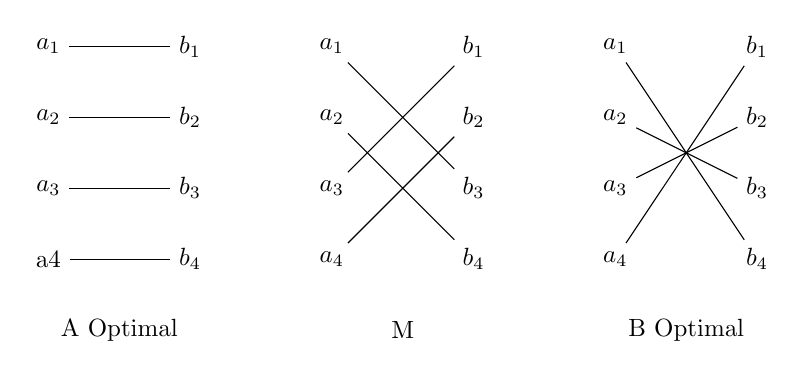
\begin{tikzpicture}[scale=0.9, every node/.style={scale=0.9}, node distance=0.8cm and 2.5cm, >=stealth]

% Left graph (A Optimal)
\node (a1) at (0,3) {$a_1$};
\node (a2) at (0,2) {$a_2$};
\node (a3) at (0,1) {$a_3$};
\node(a4) at (0,0) {a4};

\node(b1) at (2,3) {$b_1$};
\node (b2) at (2,2) {$b_2$};
\node(b3) at (2,1) {$b_3$};
\node (b4) at (2,0) {$b_4$};

\draw (a1) -- (b1);
\draw (a2) -- (b2);
\draw (a3) -- (b3);
\draw (a4) -- (b4);

\node at (1,-1) {A Optimal};

% Middle graph (M)
\node (a1m) at (4,3) {$a_1$};
\node (a2m) at (4,2) {$a_2$};
\node(a3m) at (4,1) {$a_3$};
\node (a4m) at (4,0) {$a_4$};

\node (b1m) at (6,3) {$b_1$};
\node (b2m) at (6,2) {$b_2$};
\node (b3m) at (6,1) {$b_3$};
\node(b4m) at (6,0) {$b_4$};

\draw (a1m) -- (b3m);
\draw (a2m) -- (b4m);
\draw (a3m) -- (b1m);
\draw (a4m) -- (b2m);

\node at (5,-1) {M};

% Right graph (B Optimal)
\node (a1b) at (8,3) {$a_1$};
\node(a2b) at (8,2) {$a_2$};
\node(a3b) at (8,1) {$a_3$};
\node(a4b) at (8,0) {$a_4$};

\node(b1b) at (10,3) {$b_1$};
\node (b2b) at (10,2) {$b_2$};
\node (b3b) at (10,1) {$b_3$};
\node (b4b) at (10,0) {$b_4$};

\draw (a1b) -- (b4b);
\draw (a2b) -- (b3b);
\draw (a3b) -- (b2b);
\draw (a4b) -- (b1b);

\node at (9,-1) {B Optimal};

\end{tikzpicture}
\end{center}

\end{frame}

% \begin{frame}{Properties of shortlist}
%     \begin{itemize}
%         \item All the stable mathcing of the graph is contained in the shortlist
%     \end{itemize}
% \end{frame}
% \begin{frame}{THeorem}
%     \begin{theorem}
        
%     \end{theorem}
% \end{frame}



\begin{frame}{How to Measure the Quality of a Matching?}

We measure quality based on rankings in preference lists:

\[
\begin{aligned}
    ar(i, k) &= j \quad \text{: if } k \in B \text{ is the } j^{\text{th}} \text{ choice of } i \in A \\
    br(i, k) &= j \quad \text{: if } k \in A \text{ is the } j^{\text{th}} \text{ choice of } i \in B
\end{aligned}
\]

\pause
Given a stable matching \( S = \{(a_1, b_1), (a_2, b_2), \ldots, (a_n, b_n)\} \), we define the \textbf{cost} of the matching as:

\[
c(S) = \sum_{i=1}^{n} ar(a_i, b_i) + \sum_{i=1}^{n} br(b_i, a_i)
\]

\pause
A stable matching is called \textbf{egalitarian-optimal} if it minimizes the total cost \( c(S) \).

\medskip
\textbf{Observation:} The minimum possible value of \( c(S) \) is \( 2n \), which occurs when everyone gets their first choice.
\end{frame}



\begin{frame}{Satisfaction computation}
\begin{columns}[t]
    %--- Left column: Side A Preferences
    \begin{column}{0.45\textwidth}
      \textbf{A Preferences}\\[6pt]
      \begin{tabular}{r@{: }l}
        $a_1$ & $b_1$,\,$b_3$,\,$b_2$,\,$b_4$ \\
        $a_2$ & $b_2$,\,$b_4$,\,$b_1$,\,$b_3$ \\
        $a_3$ & $b_3$,\,$b_1$,\,$b_4$,\,$b_2$ \\
        $a_4$ & $b_4$,\,$b_2$,\,$b_3$,\,$b_1$ \\
      \end{tabular}
    \end{column}

    %--- Right column: Side B Preferences
    \begin{column}{0.45\textwidth}
      \textbf{B Preferences}\\[6pt]
      \begin{tabular}{r@{: }l}
        $b_1$ & $a_4$,\,$a_3$,\,$a_2$,\,$a_1$ \\
        $b_2$ & $a_3$,\,$a_4$,\,$a_1$,\,$a_2$ \\
        $b_3$ & $a_2$,\,$a_1$,\,$a_4$,\,$a_3$ \\
        $b_4$ & $a_1$,\,$a_2$,\,$a_3$,\,$a_4$ \\
      \end{tabular}
    \end{column}
  \end{columns}
\begin{center}
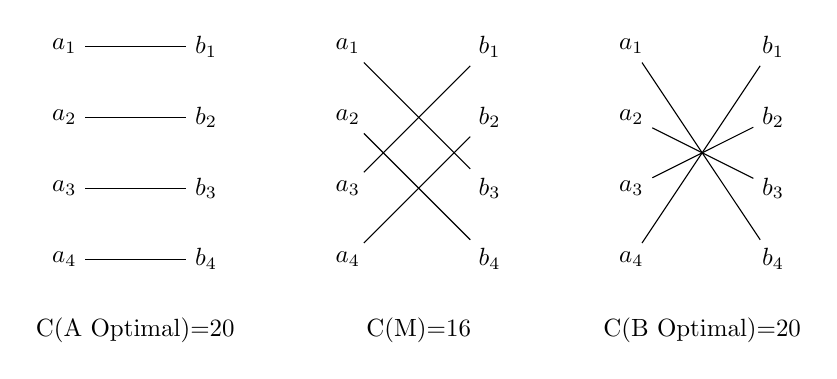
\begin{tikzpicture}[scale=0.9, every node/.style={scale=0.9}, node distance=0.8cm and 2.5cm, >=stealth]

% Left graph (A Optimal)
\node (a1) at (0,3) {$a_1$};
\node (a2) at (0,2) {$a_2$};
\node (a3) at (0,1) {$a_3$};
\node(a4) at (0,0) {$a_4$};

\node(b1) at (2,3) {$b_1$};
\node (b2) at (2,2) {$b_2$};
\node(b3) at (2,1) {$b_3$};
\node (b4) at (2,0) {$b_4$};

\draw (a1) -- (b1);
\draw (a2) -- (b2);
\draw (a3) -- (b3);
\draw (a4) -- (b4);

\node at (1,-1) {C(A Optimal)=20};

% Middle graph (M)
\node (a1m) at (4,3) {$a_1$};
\node (a2m) at (4,2) {$a_2$};
\node(a3m) at (4,1) {$a_3$};
\node (a4m) at (4,0) {$a_4$};

\node (b1m) at (6,3) {$b_1$};
\node (b2m) at (6,2) {$b_2$};
\node (b3m) at (6,1) {$b_3$};
\node(b4m) at (6,0) {$b_4$};

\draw (a1m) -- (b3m);
\draw (a2m) -- (b4m);
\draw (a3m) -- (b1m);
\draw (a4m) -- (b2m);

\node at (5,-1) {C(M)=16};

% Right graph (B Optimal)
\node (a1b) at (8,3) {$a_1$};
\node(a2b) at (8,2) {$a_2$};
\node(a3b) at (8,1) {$a_3$};
\node(a4b) at (8,0) {$a_4$};

\node(b1b) at (10,3) {$b_1$};
\node (b2b) at (10,2) {$b_2$};
\node (b3b) at (10,1) {$b_3$};
\node (b4b) at (10,0) {$b_4$};

\draw (a1b) -- (b4b);
\draw (a2b) -- (b3b);
\draw (a3b) -- (b2b);
\draw (a4b) -- (b1b);

\node at (9,-1) {C(B Optimal)=20};

\end{tikzpicture}
\end{center}

\end{frame}


\begin{frame}{Example of shortlists.}
    \begin{columns}[t]
    %--- Left column: Side A Preferences
    \begin{column}{0.45\textwidth}
      \textbf{A Preferences}\\[6pt]
      \begin{tabular}{r@{: }l}
        $a_1$ & $b_3$, $b_1$, $b_5$, $b_4$, $b_2$ \\
        $a_2$ & $b_1$, $b_3$, $b_4$, $b_5$, $b_2$ \\
        $a_3$ & $b_4$, $b_3$, $b_5$, $b_1$, $b_2$ \\
        $a_4$ & $b_5$, $b_3$, $b_1$, $b_2$, $b_4$ \\
        $a_5$ & $b_4$, $b_1$, $b_2$, $b_3$, $b_5$ \\
      \end{tabular}
    \end{column}

    %--- Right column: Side B Preferences
    \begin{column}{0.45\textwidth}
      \textbf{B Preferences}\\[6pt]
      \begin{tabular}{r@{: }l}
        $b_1$ & $a_4$, $a_3$, $a_1$, $a_2$, $a_5$ \\
        $b_2$ & $a_3$, $a_5$, $a_4$, $a_1$, $a_2$ \\
        $b_3$ & $a_5$, $a_3$, $a_2$, $a_1$, $a_4$ \\
        $b_4$ & $a_4$, $a_2$, $a_3$, $a_1$, $a_5$ \\
        $b_5$ & $a_1$, $a_5$, $a_4$, $a_3$, $a_2$ \\
      \end{tabular}
    \end{column}
  \end{columns}
\end{frame}
\begin{frame}{Example of shortlists.}
    \begin{columns}[t]
    %--- Left column: Side A Preferences
    \begin{column}{0.45\textwidth}
      \textbf{A Preferences}\\[6pt]
      \begin{tabular}{r@{: }l}
        $a_1$ & \textcolor{red}{$b_3$}, \textcolor{gray}{$b_1$, $b_5$, $b_4$, $b_2$} \\
        $a_2$ & \textcolor{red}{$b_1$}, \textcolor{gray}{$b_3$, $b_4$, $b_5$, $b_2$} \\
        $a_3$ & \textcolor{red}{$b_4$}, \textcolor{gray}{$b_3$, $b_5$, $b_1$, $b_2$} \\
        $a_4$ & \textcolor{red}{$b_5$}, \textcolor{gray}{$b_3$, $b_1$, $b_2$, $b_4$} \\
        $a_5$ & \textcolor{red}{$b_4$}, \textcolor{gray}{$b_1$, $b_2$, $b_3$, $b_5$} \\
      \end{tabular}
    \end{column}

    %--- Right column: Side B Preferences
    \begin{column}{0.45\textwidth}
      \textbf{B Preferences}\\[6pt]
      \begin{tabular}{r@{: }l}
        $b_1$ & \textcolor{gray}{$a_4$, $a_3$, $a_1$}, \textcolor{red}{$a_2$}, \textcolor{gray}{$a_5$} \\
        $b_2$ & \textcolor{gray}{$a_3$, $a_5$, $a_4$, $a_1$, $a_2$} \\
        $b_3$ & \textcolor{gray}{$a_5$, $a_3$, $a_2$}, \textcolor{red}{$a_1$}, \textcolor{gray}{$a_4$} \\
        $b_4$ & \textcolor{gray}{$a_4$, $a_2$}, \textcolor{red}{$a_3$}, \textcolor{gray}{$a_1$}, \textcolor{red}{$a_5$} \\
        $b_5$ & \textcolor{gray}{$a_1$, $a_5$}, \textcolor{red}{$a_4$}, \textcolor{gray}{$a_3$, $a_2$} \\
      \end{tabular}
    \end{column}
  \end{columns}
\end{frame}

\begin{frame}{Example of shortlists.}
    \begin{columns}[t]
    %--- Left column: Side A Preferences
    \begin{column}{0.45\textwidth}
      \textbf{A Preferences}\\[6pt]
      \begin{tabular}{r@{: }l}
        $a_1$ & \textcolor{red}{$b_3$}, \textcolor{gray}{$b_1$, $b_5$, $b_4$, $b_2$} \\
        $a_2$ & \textcolor{red}{$b_1$}, \textcolor{gray}{$b_3$, $b_4$, $b_5$, $b_2$} \\
        $a_3$ & \textcolor{red}{$b_4$}, \textcolor{gray}{$b_3$, $b_5$, $b_1$, $b_2$} \\
        $a_4$ & \textcolor{red}{$b_5$}, \textcolor{gray}{$b_3$, $b_1$, $b_2$, $b_4$} \\
        $a_5$ & \textcolor{gray}{$b_4$}, \textcolor{red}{$b_1$}, \textcolor{gray}{$b_2$, $b_3$, $b_5$} \\
      \end{tabular}
    \end{column}

    %--- Right column: Side B Preferences
    \begin{column}{0.45\textwidth}
      \textbf{B Preferences}\\[6pt]
      \begin{tabular}{r@{: }l}
        $b_1$ & \textcolor{gray}{$a_4$, $a_3$, $a_1$}, \textcolor{red}{$a_2$}, \textcolor{red}{$a_5$} \\
        $b_2$ & \textcolor{gray}{$a_3$, $a_5$, $a_4$, $a_1$, $a_2$} \\
        $b_3$ & \textcolor{gray}{$a_5$, $a_3$, $a_2$}, \textcolor{red}{$a_1$}, \textcolor{gray}{$a_4$} \\
        $b_4$ & \textcolor{gray}{$a_4$, $a_2$}, \textcolor{red}{$a_3$}, \textcolor{gray}{$a_1$, $a_5$} \\
        $b_5$ & \textcolor{gray}{$a_1$, $a_5$}, \textcolor{red}{$a_4$}, \textcolor{gray}{$a_3$, $a_2$} \\
      \end{tabular}
    \end{column}
  \end{columns}
\end{frame}

\begin{frame}{Example of shortlists.}
    \begin{columns}[t]
    %--- Left column: Side A Preferences
    \begin{column}{0.45\textwidth}
      \textbf{A Preferences}\\[6pt]
      \begin{tabular}{r@{: }l}
        $a_1$ & \textcolor{red}{$b_3$}, \textcolor{gray}{$b_1$, $b_5$, $b_4$, $b_2$} \\
        $a_2$ & \textcolor{red}{$b_1$}, \textcolor{gray}{$b_3$, $b_4$, $b_5$, $b_2$} \\
        $a_3$ & \textcolor{red}{$b_4$}, \textcolor{gray}{$b_3$, $b_5$, $b_1$, $b_2$} \\
        $a_4$ & \textcolor{red}{$b_5$}, \textcolor{gray}{$b_3$, $b_1$, $b_2$, $b_4$} \\
        $a_5$ & \textcolor{gray}{$b_4$, $b_1$}, \textcolor{red}{$b_2$}, \textcolor{gray}{$b_3$, $b_5$} \\
      \end{tabular}
    \end{column}

    %--- Right column: Side B Preferences
    \begin{column}{0.45\textwidth}
      \textbf{B Preferences}\\[6pt]
      \begin{tabular}{r@{: }l}
        $b_1$ & \textcolor{gray}{$a_4$, $a_3$, $a_1$}, \textcolor{red}{$a_2$}, \textcolor{gray}{$a_5$} \\
        $b_2$ & \textcolor{gray}{$a_3$}, \textcolor{red}{$a_5$}, \textcolor{gray}{$a_4$, $a_1$, $a_2$} \\
        $b_3$ & \textcolor{gray}{$a_5$, $a_3$, $a_2$}, \textcolor{red}{$a_1$}, \textcolor{gray}{$a_4$} \\
        $b_4$ & \textcolor{gray}{$a_4$, $a_2$}, \textcolor{red}{$a_3$}, \textcolor{gray}{$a_1$, $a_5$} \\
        $b_5$ & \textcolor{gray}{$a_1$, $a_5$}, \textcolor{red}{$a_4$}, \textcolor{gray}{$a_3$, $a_2$} \\
      \end{tabular}
    \end{column}
  \end{columns}
\end{frame}


\begin{frame}{Example of shortlists.}
    \begin{columns}[t]
    %--- Left column: Side A Preferences
    \begin{column}{0.45\textwidth}
      \textbf{A Preferences}\\[6pt]
      \begin{tabular}{r@{: }l}
        $a_1$ & \textcolor{red}{$b_3$}, \textcolor{gray}{$b_1$, $b_5$}, \textcolor{gray}{\sout{$b_4$, $b_2$}} \\
        $a_2$ & \textcolor{red}{$b_1$}, \textcolor{gray}{$b_3$, $b_4$}, \textcolor{gray}{\sout{$b_5$, $b_2$}} \\
        $a_3$ & \textcolor{red}{$b_4$}, \textcolor{gray}{$b_3$}, \textcolor{gray}{\sout{$b_5$}}, \textcolor{gray}{$b_1$, $b_2$} \\
        $a_4$ & \textcolor{red}{$b_5$}, \textcolor{gray}{\sout{$b_3$}}, \textcolor{gray}{$b_1$}, \textcolor{gray}{\sout{$b_2$}}, \textcolor{gray}{$b_4$} \\
        $a_5$ & \textcolor{gray}{\sout{$b_4$, $b_1$}}, \textcolor{red}{$b_2$}, \textcolor{gray}{$b_3$, $b_5$} \\
      \end{tabular}
    \end{column}

    %--- Right column: Side B Preferences
    \begin{column}{0.45\textwidth}
      \textbf{B Preferences}\\[6pt]
      \begin{tabular}{r@{: }l}
        $b_1$ & \textcolor{gray}{$a_4$, $a_3$, $a_1$}, \textcolor{red}{$a_2$}, \textcolor{gray}{\sout{$a_5$}} \\
        $b_2$ & \textcolor{gray}{$a_3$}, \textcolor{red}{$a_5$}, \textcolor{gray}{\sout{$a_4$, $a_1$, $a_2$}} \\
        $b_3$ & \textcolor{gray}{$a_5$, $a_3$, $a_2$}, \textcolor{red}{$a_1$}, \textcolor{gray}{\sout{$a_4$}} \\
        $b_4$ & \textcolor{gray}{$a_4$, $a_2$}, \textcolor{red}{$a_3$}, \textcolor{gray}{\sout{$a_1$, $a_5$}} \\
        $b_5$ & \textcolor{gray}{$a_1$, $a_5$}, \textcolor{red}{$a_4$}, \textcolor{gray}{\sout{$a_3$, $a_2$}} \\
      \end{tabular}
    \end{column}
  \end{columns}

  \pause
  \vspace{0.5em}
  \textbf{Cost of matching:} \( C(S) = 1 + 1 + 1 + 1 + 3 + 4 + 2 + 4 + 3 + 3 = 23 \)
\end{frame}

\begin{frame}{Shortlist}
\begin{definition}[Shortlist]
Given a stable marriage instance and a run of the Gale--Shapley algorithm (with one side proposing), the \textbf{shortlist} of an individual is the reduced preference list formed as follows:

\begin{itemize}
    \item For a proposer (A), the shortlist consists of all individuals (B) to whom (A) proposed and were not rejected, or for whom (A) remains on (B)'s preference list.
    \item For a receiver (B), the shortlist consists of all proposers (A) who are preferred over any currently matched partner, as well as the currently matched (A).
\end{itemize}
\end{definition}
\end{frame}


\begin{frame}{Property 1: Stability and Shortlists}
  \textbf{Property 1:} If \( b \) does not appear on \( a \)'s shortlist, then there is no stable matching in which \( a \) and \( b \) are partners.
\pause
  \begin{itemize}
    \item If a person is not included in the shortlist of another person, it is impossible for them to be paired in a stable matching.
    \item This ensures that only those who are "considered" can form a potential stable pair.
   \end{itemize}  
      % After running Gale-Shapley and forming mutual shortlists, the resulting reduced lists still admit exactly the same set of stable matchings as the original instance.

      % proof?
 
\end{frame}
\begin{frame}{Property 2: Symmetry of Shortlists}
  \textbf{Property 2:} \( b \) appears on \( a \)'s shortlist if and only if \( a \) appears on \( b \)'s, and \( b \) is first on \( a \)'s shortlist if and only if \( a \) is last on \( b \)'s.
\pause
  \begin{itemize}
    \item The appearance of a partner in each other's shortlist is symmetric.
    \item This implies a certain balance in how candidates are evaluated by both sides, with preferences mirroring each other.
  \end{itemize}
\end{frame}

\begin{frame}{Property 3: A-Optimal Solution}

\textbf{Property 3:} If each element in \( a \) is matched with the first choice on its shortlist, the resulting matching is stable. This is referred to as the \textbf{A-optimal} solution.
\pause
\begin{itemize}
  \item This matching is optimal for \( A \), since no element in \( A \) can be matched with a more preferred partner.
  \item Moreover, no element in \( B \) can be matched with a less preferred partner in any other stable matching.
\end{itemize}
\pause
\textbf{Key Point:} This solution guarantees maximum satisfaction for the side \( A \), while preserving stability.
\end{frame}

\begin{frame}{Property 4: B-Optimal Solution}

\textbf{Property 4:} If the roles of \( A \) and \( B \) are interchanged, and each element in \( B \) is matched with the first choice on its (B-oriented) shortlist, then the resulting matching is stable. This is called the \textbf{B-optimal} solution.
\pause
\begin{itemize}
  \item This matching is optimal for \( B \), since no element in \( B \) can be matched with a more preferred partner.
  \item Conversely, no element in \( A \) can be matched with a less preferred partner in any other stable matching.
\end{itemize}
\pause
\textbf{Key Point:} This solution maximizes satisfaction for \( B \), while maintaining stability under the reversed roles.
\end{frame}



\begin{frame}{Shortlists After Gale--Shapley}
\begin{itemize}
  % \item After the Gale--Shapley algorithm terminates, each individual’s shortlist contains all partners they could be matched with in some stable matching.
  \item The proposer ends up with their best possible stable partner.
  \pause
  \item The receiver is matched with their most preferred option among those who proposed.\pause
  \item All removed pairs can never appear in any stable matching.
\end{itemize}
\pause
\textbf{Conclusion:} The mutual shortlists preserve the full set of possible stable matchings.
\end{frame}
\begin{frame}{Singleton Set}
    After matching, the shortlist can be divided into two sets:
    \begin{itemize}
        \item A set of elements containing only the currently matched partner in the preference list, known as the singleton preference list.
        \item A set of elements containing more than one element in the preference list.
    \end{itemize}
\end{frame}


\begin{frame}{Rotation}
  \begin{definition}[Rotation]
    % A \textbf{rotation} \( p = (a_0, b_0), (a_1, b_1), \dots, (a_{r-1}, b_{r-1}) \) is a sequence of matched pairs where each \( a_i \) is matched to \( b_i \), and the pairs follow a cyclic order.
    A \textbf{rotation} \( p = (a_0, b_0), (a_1, b_1), \dots, (a_{r-1}, b_{r-1}) \) is a sequence of matched pairs where \( b_i \) is first in \( a_i \)'s shortlist, and \( b_{(i+1) \bmod r} \) is second in \( a_i \)'s shortlist.


    
    In the elimination process:
    \begin{itemize}
      \item For each \( i \), the successor \( x \) of \( a_{i-1} \) in \( b_i \)'s shortlist is removed.
      \item The corresponding appearance of \( b_i \) is removed from \( x \)'s preference list.
    \end{itemize}
    The rotation \( p \) is eliminated when this process is applied for all \( i \), \( 0 \leq i \leq r-1 \), with \( i-1 \) taken modulo \( r \).
  \end{definition}
\end{frame}

\begin{frame}{Weight of a Rotation}
    Given a rotation \( \rho = (a_0, b_0), \ldots, (a_{r-1}, b_{r-1}) \) in a stable matching instance,  
    we define its weight \( w(\rho) \) as:
    
    \[
    w(\rho) = \sum_{i=0}^{r-1} \left( \text{ar}(a_i, b_i) - \text{ar}(a_i, b_{(i+1) \bmod r}) \right)
    + \sum_{i=0}^{r-1} \left( \text{br}(b_i, a_i) - \text{br}(b_i, a_{(i-1) \bmod r}) \right)
    \]

    \pause
    This captures the total change in satisfaction for both sides when rotation \( \rho \) is eliminated.
\end{frame}



\begin{frame}{Rotation}
\begin{center}
    \begin{tikzpicture}

% Nodes for A
\node at (0,4) (a1) {$a_i$};
\node at (0,3) (a2) {$a_j$};
\node at (0,2) (a3) {$a_k$};
\node at (0,1) (a4) {$a_l$};
\node at (0,0) (a5) {$a_m$};

% Nodes for B
\node at (4,4) (b1) {$b_n$};
\node at (4,3) (b2) {$b_o$};
\node at (4,2) (b3) {$b_p$};
\node at (4,1) (b4) {$b_q$};
\node at (4,0) (b5) {$b_r$};

% --- Frame 1: original red edges only
    \draw[red, thick, shorten <= 0.3cm, shorten >= 0.3cm] (a1) -- (b1) node[pos=0.1, left,yshift=0.2cm] {2} node[pos=0.9, right,yshift=0.2cm] {10};
\only<1>{
    \draw[red, thick, shorten <= 0.3cm, shorten >= 0.3cm] (a2) -- (b2) node[pos=0.1, left,yshift=0.2cm] {3} node[pos=0.9, right] {9};
    \draw[red, thick, shorten <= 0.3cm, shorten >= 0.3cm] (a3) -- (b3) node[pos=0.1, left,yshift=0.2cm] {1} node[pos=0.9, right] {7};
    \draw[red, thick, shorten <= 0.3cm, shorten >= 0.3cm] (a4) -- (b4) node[pos=0.1, left,yshift=0.2cm] {2} node[pos=0.9, right,yshift=-0.2cm] {5};
    \draw[red, thick, shorten <= 0.3cm, shorten >= 0.3cm] (a5) -- (b5) node[pos=0.1, left,yshift=-0.2cm] {2} node[pos=0.85, right,yshift=-0.2cm] {6};
}

% --- Frame 2: original red + new blue edges
\only<2->{
    \draw[blue, thick, shorten <= 0.2cm, shorten >= 0.2cm] (a1) -- (b2) node[pos=0.1, left] {5} node[pos=0.9, right,yshift=0.2cm,xshift=-0.2cm] {6};}
\only<2>{
    % Red edges
    \draw[red, thick, shorten <= 0.3cm, shorten >= 0.3cm] (a1) -- (b1) node[pos=0.1, left,yshift=0.2cm] {2} node[pos=0.9, right,yshift=0.2cm] {10};
    \draw[red, thick, shorten <= 0.3cm, shorten >= 0.3cm] (a2) -- (b2) node[pos=0.1, left,yshift=0.2cm] {3} node[pos=0.9, right] {9};
    \draw[red, thick, shorten <= 0.3cm, shorten >= 0.3cm] (a3) -- (b3) node[pos=0.1, left,yshift=0.2cm] {1} node[pos=0.9, right] {7};
    \draw[red, thick, shorten <= 0.3cm, shorten >= 0.3cm] (a4) -- (b4) node[pos=0.1, left,yshift=0.2cm] {2} node[pos=0.9, right,yshift=-0.2cm] {5};
    \draw[red, thick, shorten <= 0.3cm, shorten >= 0.3cm] (a5) -- (b5) node[pos=0.1, left,yshift=-0.2cm] {2} node[pos=0.85, right,yshift=-0.2cm] {6};

    % Blue edges
    \draw[blue, thick, shorten <= 0.2cm, shorten >= 0.2cm] (a2) -- (b3) node[pos=0.1, left] {6} node[pos=0.9, right,yshift=0.2cm] {6};
    \draw[blue, thick, shorten <= 0.2cm, shorten >= 0.2cm] (a3) -- (b4) node[pos=0.1, left] {2} node[pos=0.9, right,yshift=0.2cm,xshift=-0.2cm] {3};
    \draw[blue, thick, shorten <= 0.2cm, shorten >= 0.2cm] (a4) -- (b5) node[pos=0.1, left] {4} node[pos=0.9, right,yshift=0.2cm,xshift=-0.2cm] {2};
    \draw[blue, thick] (a5) -- (b2) node[pos=0.1, left,yshift=-0.4cm] {5} node[pos=0.9, right,yshift=0.2cm,xshift=-0.2cm] {7};
}

% --- Frame 3 and onward: only blue edges shown as red
\only<3->{
    \draw[red, thick, shorten <= 0.2cm, shorten >= 0.2cm] (a2) -- (b3) node[pos=0.1, left] {6} node[pos=0.9, right,yshift=0.2cm] {6};
    \draw[red, thick, shorten <= 0.2cm, shorten >= 0.2cm] (a3) -- (b4) node[pos=0.1, left] {2} node[pos=0.9, right,yshift=0.2cm,xshift=-0.2cm] {3};
    \draw[red, thick, shorten <= 0.2cm, shorten >= 0.2cm] (a4) -- (b5) node[pos=0.1, left] {4} node[pos=0.9, right,yshift=0.2cm,xshift=-0.2cm] {2};
    \draw[red, thick] (a5) -- (b2) node[pos=0.1, left,yshift=-0.4cm] {5} node[pos=0.9, right,yshift=0.2cm,xshift=-0.2cm] {7};
}

\end{tikzpicture}

\only<1>{Current matching in some arbitary graph}
\only<2>{

Rotation ($a_j$,$b_o$),($a_k$,$b_p$),($a_l$,$b_q$),($a_m$,$b_r$)
}
\only<3>{
  
  \[
   \text{\textbf{Weight of this rotation:}} (3 - 6) + (1 - 2) + (2 - 4) + (5 - 2) + (9 - 7) + (7 - 6) + (5 - 3) + (6 - 2) = 6
  \]
}

\end{center}
\end{frame}

\begin{frame}{Rotation Elimination}
  A rotation \( \rho = (a_0, b_0), (a_1, b_1), \ldots, (a_{r-1}, b_{r-1}) \) is said to be \textbf{eliminated} if:
  \begin{itemize}
    \item For each \( i \) (where \( 0 \leq i < r \)), every successor \( x \) of \( a_{i-1} \) (modulo \( r \)) in \( b_i \)'s shortlist is removed.
    \item The corresponding appearance of \( b_i \) is also removed from each such \( x \)'s shortlist.
    \item These deletions remove all potential for \( a_{i-1} \) and \( b_i \) to form a better pair in the future.
  \end{itemize}
  The rotation \( \rho \) is then said to be the \textbf{eliminating rotation} for all such removed pairs.
\end{frame}

\begin{frame}{Elimination Prevents Blocking Pairs}
  Eliminating a rotation ensures stability by preventing blocking pairs:
  \begin{itemize}
    \item A blocking pair \((a, b)\) exists if both prefer each other over their current partners.
    \item After eliminating a rotation, successors of each \( a_{i-1} \) are removed from \( b_i \)'s list, and vice versa.
    \item This ensures that neither \( a_{i-1} \) nor \( b_i \) can later form a more preferred match.
    \item Therefore, no new blocking pairs can arise from these individuals.
  \end{itemize}
\end{frame}

% \begin{frame}{Argument for Stability}
%   \begin{itemize}
%     \item The individuals involved are removed from each other's shortlists.
%     \item They can no longer form a blocking pair because they are no longer considered in each other's preferences.
%     \item Thus, the matching remains stable after each elimination.
%   \end{itemize}
% \end{frame}

% \begin{frame}{Conclusion}
%   After elimination of each rotation, the matching remains stable because:
%   \begin{itemize}
%     \item No new blocking pairs are introduced, as all potential alternatives are removed.
%     \item Each individual is either matched to their current partner or no longer considers any new matches that could lead to instability.
%   \end{itemize}
%   Therefore, the matching after rotation is stable.
% \end{frame}

\begin{frame}{Shortlists After Gale-Shapley}

  \begin{columns}[t]
    % Left column: A Preferences
    \begin{column}{0.48\textwidth}
      \textbf{A Preferences}\\[6pt]
      \begin{tabular}{r@{: }l}
        $a_1$ & \textcolor{red}{$b_3$}, \textcolor{gray}{$b_1$}, \textcolor{gray}{$b5$}, \sout{\textcolor{gray}{$b_4$}}, \sout{\textcolor{gray}{$b_2$}} \\
        $a_2$ & \textcolor{red}{$b_1$}, \textcolor{gray}{$b_3$}, \textcolor{gray}{$b_4$}, \sout{\textcolor{gray}{$b5$}}, \sout{\textcolor{gray}{$b_2$}} \\
        $a_3$ & \textcolor{red}{$b_4$}, \textcolor{gray}{$b_3$}, \sout{\textcolor{gray}{$b5$}}, \textcolor{gray}{$b_1$}, \textcolor{gray}{$b_2$} \\
        $a_4$ & \textcolor{red}{$b5$}, \sout{\textcolor{gray}{$b_3$}}, \textcolor{gray}{$b_1$}, \sout{\textcolor{gray}{$b_2$}}, \textcolor{gray}{$b_4$} \\
        $a_5$ & \sout{\textcolor{gray}{$b_4$}}, \sout{\textcolor{gray}{$b_1$}}, \textcolor{red}{$b_2$}, \textcolor{gray}{$b_3$}, \textcolor{gray}{$b5$} \\
      \end{tabular}
    \end{column}

    % Right column: B Preferences
    \begin{column}{0.48\textwidth}
      \textbf{B Preferences}\\[6pt]
      \begin{tabular}{r@{: }l}
        b1 & \textcolor{gray}{$a_4$}, \textcolor{gray}{$a_3$}, \textcolor{gray}{$a_1$}, \textcolor{red}{$a_2$}, \sout{\textcolor{gray}{$a_5$}} \\
        b2 & \textcolor{gray}{$a_3$}, \textcolor{red}{$a_5$}, \sout{\textcolor{gray}{$a_4$}}, \sout{\textcolor{gray}{$a_1$}}, \sout{\textcolor{gray}{$a_2$}} \\
        b3 & \textcolor{gray}{$a_5$}, \textcolor{gray}{$a_3$}, \textcolor{gray}{$a_2$}, \textcolor{red}{$a_1$}, \sout{\textcolor{gray}{$a_4$}} \\
        b4 & \textcolor{gray}{$a_4$}, \textcolor{gray}{$a_2$}, \textcolor{red}{$a_3$}, \sout{\textcolor{gray}{$a_1$}}, \sout{\textcolor{gray}{$a_5$}} \\
        b5 & \textcolor{gray}{$a_1$}, \textcolor{gray}{$a_5$}, \textcolor{red}{$a_4$}, \sout{\textcolor{gray}{$a_3$}}, \sout{\textcolor{gray}{$a_2$}} \\
      \end{tabular}
    \end{column}
  \end{columns}

  \vspace{1em}
  \pause
  \textbf{Rotation Identified:} $(a_1, b_3), (a_2, b_1)$
\end{frame}

\begin{frame}{Shortlist}
Eliminating rotation \( (a_1, b_3), (a_2, b_1) \)

\vspace{1em}
\begin{columns}[t]
  %--- Left column: Side A Preferences
  \begin{column}{0.45\textwidth}
    \textbf{A Preferences}\\[6pt]
    \begin{tabular}{r@{: }l}
      $a_1$ & \sout{\textcolor{green}{$b_3$}}, \textcolor{red}{$b_1$}, \textcolor{gray}{$b_5$}, \sout{\textcolor{gray}{$b_4$}}, \sout{\textcolor{gray}{$b_2$}} \\
      $a_2$ & \sout{\textcolor{green}{$b_1$}}, \textcolor{red}{$b_3$}, \textcolor{gray}{$b_4$}, \textcolor{gray}{$b_5$}, \sout{\textcolor{gray}{$b_2$}} \\
      $a_3$ & \textcolor{red}{$b_4$}, \textcolor{gray}{$b_3$}, \sout{\textcolor{gray}{$b_5$}}, \textcolor{gray}{$b_1$}, \textcolor{gray}{$b_2$} \\
      $a_4$ & \textcolor{red}{$b_5$}, \sout{\textcolor{gray}{$b_3$}}, \textcolor{gray}{$b_1$}, \sout{\textcolor{gray}{$b_2$}}, \textcolor{gray}{$b_4$} \\
      $a_5$ & \sout{\textcolor{gray}{$b_4$}}, \sout{\textcolor{gray}{$b_1$}}, \textcolor{red}{$b_2$}, \textcolor{gray}{$b_3$}, \textcolor{gray}{$b_5$} \\
    \end{tabular}
  \end{column}

  %--- Right column: Side B Preferences
  \begin{column}{0.45\textwidth}
    \textbf{B Preferences}\\[6pt]
    \begin{tabular}{r@{: }l}
      $b_1$ & \textcolor{gray}{$a_4$}, \textcolor{gray}{$a_3$}, \textcolor{red}{$a_1$}, \sout{\textcolor{green}{$a_2$}}, \sout{\textcolor{gray}{$a_5$}} \\
      $b_2$ & \textcolor{gray}{$a_3$}, \textcolor{red}{$a_5$}, \sout{\textcolor{gray}{$a_4$}}, \sout{\textcolor{gray}{$a_1$}}, \sout{\textcolor{gray}{$a_2$}} \\
      $b_3$ & \textcolor{gray}{$a_5$}, \textcolor{gray}{$a_3$}, \textcolor{red}{$a_2$}, \sout{\textcolor{green}{$a_1$}}, \sout{\textcolor{gray}{$a_4$}} \\
      $b_4$ & \textcolor{gray}{$a_4$}, \textcolor{gray}{$a_2$}, \textcolor{red}{$a_3$}, \sout{\textcolor{gray}{$a_1$}}, \sout{\textcolor{gray}{$a_5$}} \\
      $b_5$ & \textcolor{gray}{$a_1$}, \textcolor{gray}{$a_5$}, \textcolor{red}{$a_4$}, \sout{\textcolor{gray}{$a_3$}}, \sout{\textcolor{gray}{$a_2$}} \\
    \end{tabular}
  \end{column}
\end{columns}

\vspace{1em}
\pause
\textbf{Weight of rotation \( \rho_1 \):} \( (-1-1) + (1+1) = 0 \)

\pause
\textbf{Two new rotations were exposed:} 
\[
(a_1, b_1), (a_4, b_5) \quad \text{and} \quad (a_3, b_4), (a_2, b_3)
\]

\pause
Note that rotations are not necessarily of size 2.
\end{frame}


\begin{frame}{Shortlist}
Eliminating rotation \( (a_1, b_1), (a_4, b_5) \)

\vspace{1em}
\begin{columns}[t]
  %--- Left column: Side A Preferences
  \begin{column}{0.45\textwidth}
    \textbf{A Preferences}\\[6pt]
    \begin{tabular}{r@{: }l}
      $a_1$ & \sout{\textcolor{gray}{$b_3$}, \textcolor{green}{$b_1$}}, \textcolor{red}{$b_5$}, \sout{\textcolor{gray}{$b_4$}}, \sout{\textcolor{gray}{$b_2$}} \\
      $a_2$ & \sout{\textcolor{gray}{$b_1$}}, \textcolor{red}{$b_3$}, \textcolor{gray}{$b_4$}, \sout{\textcolor{gray}{$b_5$}}, \sout{\textcolor{gray}{$b_2$}} \\
      $a_3$ & \textcolor{red}{$b_4$}, \textcolor{gray}{$b_3$}, \sout{\textcolor{gray}{$b_5$}}, \sout{\textcolor{gray}{$b_1$}}, \textcolor{gray}{$b_2$} \\
      $a_4$ & \sout{\textcolor{green}{$b_5$}, \textcolor{gray}{$b_3$}}, \textcolor{red}{$b_1$}, \sout{\textcolor{gray}{$b_2$}}, \textcolor{gray}{$b_4$} \\
      $a_5$ & \sout{\textcolor{gray}{$b_4$}, \textcolor{gray}{$b_1$}}, \textcolor{red}{$b_2$}, \textcolor{gray}{$b_3$}, \sout{\textcolor{gray}{$b_5$}} \\
    \end{tabular}
  \end{column}

  %--- Right column: Side B Preferences
  \begin{column}{0.45\textwidth}
    \textbf{B Preferences}\\[6pt]
    \begin{tabular}{r@{: }l}
      $b_1$ & \textcolor{red}{$a_4$}, \sout{\textcolor{gray}{$a_3$}, \textcolor{green}{$a_1$}, \textcolor{gray}{$a_2$}, \textcolor{gray}{$a_5$}} \\
      $b_2$ & \textcolor{gray}{$a_3$}, \textcolor{red}{$a_5$}, \sout{\textcolor{gray}{$a_4$}, \textcolor{gray}{$a_1$}, \textcolor{gray}{$a_2$}} \\
      $b_3$ & \textcolor{gray}{$a_5$}, \textcolor{gray}{$a_3$}, \textcolor{red}{$a_2$}, \sout{\textcolor{gray}{$a_1$}, \textcolor{gray}{$a_4$}} \\
      $b_4$ & \textcolor{gray}{$a_4$}, \textcolor{gray}{$a_2$}, \textcolor{red}{$a_3$}, \sout{\textcolor{gray}{$a_1$}, \textcolor{gray}{$a_5$}} \\
      $b_5$ & \textcolor{red}{$a_1$}, \sout{\textcolor{gray}{$a_5$}, \textcolor{green}{$a_4$}, \textcolor{gray}{$a_3$}, \textcolor{gray}{$a_2$}} \\
    \end{tabular}
  \end{column}
\end{columns}


\vspace{1em}
\pause
\textbf{Weight of rotation \( \rho_2 \):} \( (-1 -2) + (2 + 2) = 1 \)

\pause
\textbf{No new rotation was exposed.}

\pause
Now we observe that \( a_1 \),\( b_1 \) and \( b_5 \) have been removed from everyone other than their matched partner.\\
Hence, no future rotations can involve these.

\end{frame}


\begin{frame}{Shortlist}
Eliminating rotation \( (a_2, b_3), (a_3, b_4) \)

\vspace{1em}
\begin{columns}[t]
  %--- Left column: Side A Preferences
  \begin{column}{0.45\textwidth}
    \textbf{A Preferences}\\[6pt]
    \begin{tabular}{r@{: }l}
      $a_1$ & \sout{\textcolor{gray}{$b_3$}, \textcolor{gray}{$b_1$}}, \textcolor{red}{$b_5$}, \sout{\textcolor{gray}{$b_4$}, \textcolor{gray}{$b_2$}} \\
      $a_2$ & \sout{\textcolor{gray}{$b_1$}, \textcolor{green}{$b_3$}}, \textcolor{red}{$b_4$}, \sout{\textcolor{gray}{$b_5$}, \textcolor{gray}{$b_2$}} \\
      $a_3$ & \sout{\textcolor{green}{$b_4$}}, \textcolor{red}{$b_3$}, \sout{\textcolor{gray}{$b_5$}, \textcolor{gray}{$b_1$}}, \textcolor{gray}{$b_2$} \\
      $a_4$ & \sout{\textcolor{gray}{$b_5$}, \textcolor{gray}{$b_3$}}, \textcolor{red}{$b_1$}, \sout{\textcolor{gray}{$b_2$}}, \textcolor{gray}{$b_4$} \\
      $a_5$ & \sout{\textcolor{gray}{$b_4$}, \textcolor{gray}{$b_1$}}, \textcolor{red}{$b_2$}, \textcolor{gray}{$b_3$}, \sout{\textcolor{gray}{$b_5$}} \\
    \end{tabular}
  \end{column}

  %--- Right column: Side B Preferences
  \begin{column}{0.45\textwidth}
    \textbf{B Preferences}\\[6pt]
    \begin{tabular}{r@{: }l}
      $b_1$ & \textcolor{red}{$a_4$}, \sout{\textcolor{gray}{$a_3$}, \textcolor{gray}{$a_1$}, \textcolor{gray}{$a_2$}, \textcolor{gray}{$a_5$}} \\
      $b_2$ & \textcolor{gray}{$a_3$}, \textcolor{red}{$a_5$}, \sout{\textcolor{gray}{$a_4$}, \textcolor{gray}{$a_1$}, \textcolor{gray}{$a_2$}} \\
      $b_3$ & \textcolor{gray}{$a_5$}, \textcolor{red}{$a_3$}, \sout{\textcolor{green}{$a_2$}, \textcolor{gray}{$a_1$}, \textcolor{gray}{$a_4$}} \\
      $b_4$ & \textcolor{gray}{$a_4$}, \textcolor{red}{$a_2$}, \sout{\textcolor{green}{$a_3$}, \textcolor{gray}{$a_1$}, \textcolor{gray}{$a_5$}} \\
      $b_5$ & \textcolor{red}{$a_1$}, \sout{\textcolor{gray}{$a_5$}, \textcolor{gray}{$a_4$}, \textcolor{gray}{$a_3$}, \textcolor{gray}{$a_2$}} \\
    \end{tabular}
  \end{column}
\end{columns}

\vspace{1em}
\pause
\textbf{Weight of rotation \( \rho_3 \):} \( (-1-1) + (1+1) = 0 \)

\pause
\textbf{New rotation exposed:} 
\[
(a_3,b_3), (a_5,b_2)
\]
\end{frame}
\begin{frame}{Shortlist}
Eliminating rotation \( (a_3,b_3), (a_5,b_2) \)

\vspace{1em}
\begin{columns}[t]
  %--- Left column: Side A Preferences
  \begin{column}{0.45\textwidth}
    \textbf{A Preferences}\\[6pt]
    \begin{tabular}{r@{: }l}
      $a_1$ & \sout{\textcolor{gray}{$b_3$}, \textcolor{gray}{$b_1$}}, \textcolor{red}{$b_5$}, \sout{\textcolor{gray}{$b_4$}, \textcolor{gray}{$b_2$}} \\
      $a_2$ & \sout{\textcolor{gray}{$b_1$}, \textcolor{gray}{$b_3$}}, \textcolor{red}{$b_4$}, \sout{\textcolor{gray}{$b_5$}, \textcolor{gray}{$b_2$}} \\
      $a_3$ & \sout{\textcolor{gray}{$b_4$}, \textcolor{green}{$b_3$}, \textcolor{gray}{$b_5$}, \textcolor{gray}{$b_1$}}, \textcolor{red}{$b_2$} \\
      $a_4$ & \sout{\textcolor{gray}{$b_5$}, \textcolor{gray}{$b_3$}}, \textcolor{red}{$b_1$}, \sout{\textcolor{gray}{$b_2$}}, \textcolor{gray}{$b_4$} \\
      $a_5$ & \sout{\textcolor{gray}{$b_4$}, \textcolor{gray}{$b_1$}, \textcolor{green}{$b_2$}}, \textcolor{red}{$b_3$}, \sout{\textcolor{gray}{$b_5$}} \\
    \end{tabular}
  \end{column}

  %--- Right column: Side B Preferences
  \begin{column}{0.45\textwidth}
    \textbf{B Preferences}\\[6pt]
    \begin{tabular}{r@{: }l}
      $b_1$ & \textcolor{red}{$a_4$}, \sout{\textcolor{gray}{$a_3$}, \textcolor{gray}{$a_1$}, \textcolor{gray}{$a_2$}, \textcolor{gray}{$a_5$}} \\
      $b_2$ & \textcolor{red}{$a_3$}, \sout{\textcolor{green}{$a_5$}, \textcolor{gray}{$a_4$}, \textcolor{gray}{$a_1$}, \textcolor{gray}{$a_2$}} \\
      $b_3$ & \textcolor{red}{$a_5$}, \sout{\textcolor{green}{$a_3$}, \textcolor{gray}{$a_2$}, \textcolor{gray}{$a_1$}, \textcolor{gray}{$a_4$}} \\
      $b_4$ & \textcolor{gray}{$a_4$}, \textcolor{red}{$a_2$}, \sout{\textcolor{gray}{$a_3$}, \textcolor{gray}{$a_1$}, \textcolor{gray}{$a_5$}} \\
      $b_5$ & \textcolor{red}{$a_1$}, \sout{\textcolor{gray}{$a_5$}, \textcolor{gray}{$a_4$}, \textcolor{gray}{$a_3$}, \textcolor{gray}{$a_2$}} \\
    \end{tabular}
  \end{column}
\end{columns}


\vspace{1em}
\pause
\textbf{Weight of the rotation \( \rho_4 \):} \( (-3 - 1) + (1 + 1) = -2 \)

\pause
\textbf{Reached B optimal matching.}

\pause
\textbf{No more rotations possible.}
\end{frame}

\begin{frame}{Property}
    \begin{theorem}
        Every stable matching can be obtained by starting from the
shortlists and eliminating some sequence of zero or more exposed
rotations.
    \end{theorem}
\end{frame}


\begin{frame}{Number of Rotations}
Although a stable marriage instance with \( n \) A and \( n \) B can have exponentially many stable matchings, the number of \textbf{rotations} is bounded by \( n^2 \).
\pause
\medskip

This is because each pair \( (a, b) \) can appear in at most one rotation, and there are only \( n^2 \) such possible pairs in total.

Also no pair is eliminated more than once
\end{frame}








\begin{frame}{Explicit Predecessor and the Rotation Poset}
A rotation \( \pi \) is called an \textbf{explicit predecessor} of the rotation
\[
\rho = (a_0, b_0), (a_1, b_1), \dots, (a_{r-1}, b_{r-1})
\]
if, for some index \( i \in [0, r - 1] \) and some \( x \in B \) with \( x \ne b_i \):
\begin{itemize}
  \item The rotation \( \pi \) is the \textit{eliminating rotation} for the pair \( (a_i, x) \), and
  \item \( a_i \) prefers \( x \) over \( b_{i+1} \).
\end{itemize}
\pause
\medskip

The \textbf{rotation poset} for a problem instance is a partially ordered set where:
\[
\alpha <  \rho \iff \text{\( \alpha \) must be eliminated before \( \rho \) becomes exposed.}
\]

\medskip

A subset \( C \subseteq P \), where \( P = (I, \leq) \) is a poset, is called a \textit{closed set} if:
\[
\rho \in C,\ \pi<  \rho \Rightarrow \pi \in C.
\]
That is, all predecessors of any element in \( C \) must also lie in \( C \).
\end{frame}



\begin{frame}{Rotation Poset}
$\pi$ is an immediate predecessor of $\rho$ if 
\[
 \pi< \rho \quad \text{and there is no } \sigma \text{ such that } \pi < \sigma < \rho.
\]

\pause
\begin{tabular}{>{\arraybackslash}m{6cm} >{\arraybackslash}m{6cm}}
\toprule
\textbf{Rotation} & \textbf{Immediate Predecessors} \\
\midrule
$\rho_1 = (a1,b3),\ (a2,b1)$ & --- \\
$\rho_2 = (a1,b1),\ (a4,b5)$ & $\rho_1$ \\
$\rho_3 = (a2,b3),\ (a3,b4)$ & $\rho_1$ \\
$\rho_4 = (a3,b3),\ (a5,b2)$ & $\rho_2,\ \rho_3$ \\
\bottomrule
\end{tabular}
\end{frame}
\begin{frame}{Rotation Poset}
\centering
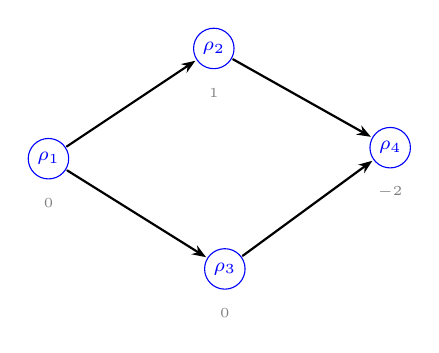
\begin{tikzpicture}[line cap=round,line join=round,scale=1.4]

% Arrows involving rho_4, rho_7, rho_8, rho_9
\draw[-{Stealth[length=5pt]}, thick, shorten >=8pt, shorten <=8pt] (-1.3,3.1) -- (0.2,4.1); % rho_4 → rho_7
\draw[-{Stealth[length=5pt]}, thick, shorten >=8pt, shorten <=8pt] (-1.3,3.1) -- (0.3,2.1); % rho_4 → rho_8
\draw[-{Stealth[length=5pt]}, thick, shorten >=8pt, shorten <=8pt] (0.2,4.1) -- (1.8,3.2);  % rho_7 → rho_9
\draw[-{Stealth[length=5pt]}, thick, shorten >=8pt, shorten <=8pt] (0.3,2.1) -- (1.8,3.2);  % rho_8 → rho_9

% Nodes
\begin{scriptsize}
\foreach \x/\y/\label/\weight in {
  -1.3/3.1/\rho_1/0,
  0.2/4.1/\rho_2/1,
  0.3/2.1/\rho_3/0,
  1.8/3.2/\rho_4/-2
} {
  \node[draw=blue, circle, inner sep=2pt, text=blue] at (\x,\y) {$\label$};
  \node[gray] at (\x,\y-0.4) {\tiny $\weight$};
}
\end{scriptsize}

\end{tikzpicture}
\end{frame}
\begin{frame}{Why always DAG?}
A \textbf{rotation poset} captures dependencies between rotations:  
$\rho_1 < \rho_2$ means $\rho_1$ must be eliminated before $\rho_2$ becomes exposed.
\pause
\medskip

\textbf{Why is it always a DAG?}
\begin{itemize}
    \item The "$<$" relation is a strict partial order.\pause
    \item A cycle would imply a set of rotations must all come before each other $\Rightarrow$ contradiction.\pause
    \item In stable matching, each eliminated rotation strictly reduces the possible matchings.\pause
    \item After eliminating a rotation:
    \begin{itemize}
        \item Each $A$ removes all partners \textbf{before} the newly matched one in her list.
        \item Each $B$ removes all partners \textbf{after} the newly matched one in his list.
    \end{itemize}\pause
    \item This pruning ensures no earlier rotation can become exposed again.\pause
    \item $\Rightarrow$ No cyclic dependencies possible $\Rightarrow$ Always a DAG.
\end{itemize}
\end{frame}





\begin{frame}{Corollary}

    Let \( S \) be the stable matching obtained by eliminating the sequence of rotations \( \rho_1, \ldots, \rho_k \) from the shortlists of a stable marriage instance.

    \pause
    Then,
    \[
        c(S) = c(S_0) - \sum_{i=1}^{k} w(\rho_i)
    \]
    where \( c(S_0) \) is the cost of the initial stable matching (e.g., A-optimal).

    \pause
    Therefore, to find an optimal stable matching, it suffices to construct a closed subset of the rotation poset with the \textbf{maximum total weight}.

    \pause
    \begin{example}
        The set \( \{\rho_1, \rho_2\} \) forms a closed subset with total weight \( +1 \).
    \end{example}

\end{frame}


\begin{frame}{Finding maximum weight closed subset of $P$}
We construct an \( s \)--\( t \) flow graph on the poset \( P \) as follows:

\begin{itemize}
    \item Add a source node \( s \) and a sink node \( t \) to the graph.
    
    \item For every \textbf{negative-weight} node \( \rho_i \), add a directed edge from \( s \) to \( \rho_i \) with capacity:
    \[
    \text{capacity}(s, \rho_i) = |w(\rho_i)|
    \]
    
    \item For every \textbf{positive-weight} node \( \rho_j \), add a directed edge from \( \rho_j \) to \( t \) with capacity:
    \[
    \text{capacity}(\rho_j, t) = w(\rho_j)
    \]
    
    \item Set the capacity of every original edge in \( P \) (i.e., edges that represent ordering constraints) to \( \infty \).
\end{itemize}
\end{frame}

\begin{frame}{Theorem: Closed Subsets via Min-Cut}
\begin{theorem}
Let \( X \) be the set of edges crossing a minimum \( s \)-\( t \) cut in the flow network \( P(s, t) \), with total capacity \( w(X) \).

\medskip

Then, the positive nodes in the maximum-weight closed subset of \( P' \) are:
\begin{itemize}
  \item Exactly those positive nodes whose edges into \( t \) are \textbf{not} in the cut \( X \),
  \item Along with all nodes that can reach them in \( P' \) (i.e., their predecessors).
\end{itemize}

\medskip

These nodes collectively form a \textbf{maximum-weight closed subset} in \( P \).
\end{theorem}
\end{frame}



\begin{frame}{Rotation Poset}
    \centering
    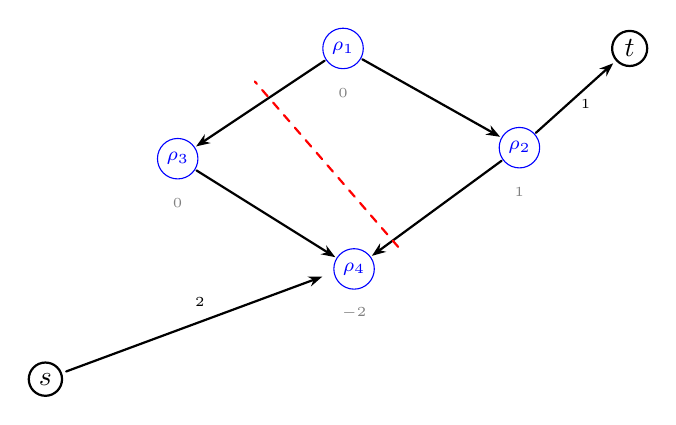
\begin{tikzpicture}[line cap=round,line join=round,scale=1.4]
    
    % Arrows between rotation nodes
    \draw[-{Stealth[length=5pt]}, thick, shorten >=8pt, shorten <=8pt](0.2,4.1)-- (-1.3,3.1) ; % rho_1 → rho_2
    \draw[-{Stealth[length=5pt]}, thick, shorten >=8pt, shorten <=8pt] (-1.3,3.1) -- (0.3,2.1); % rho_1 → rho_3
    \draw[-{Stealth[length=5pt]}, thick, shorten >=8pt, shorten <=8pt] (0.2,4.1) -- (1.8,3.2);  % rho_2 → rho_4
    \draw[-{Stealth[length=5pt]}, thick, shorten >=8pt, shorten <=8pt] (1.8,3.2)--(0.3,2.1) ;  % rho_3 → rho_4
    
    % Nodes
    \begin{scriptsize}
    \foreach \x/\y/\label/\weight in {
      -1.3/3.1/\rho_3/0,
      0.2/4.1/\rho_1/0,
      0.3/2.1/\rho_4/-2,
      1.8/3.2/\rho_2/1
    } {
      \node[draw=blue, circle, inner sep=2pt, text=blue] at (\x,\y) {$\label$};
      \node[gray] at (\x,\y-0.4) {\tiny $\weight$};
    }
    \end{scriptsize}
    
    % s and t nodes
    \node[draw=black, circle, inner sep=2pt, text=black, thick] at (-2.5,1.1) {$s$};
    \node[draw=black, circle, inner sep=2pt, text=black, thick] at (2.8,4.1) {$t$};
    
    % s → rho_4
    \draw[-{Stealth[length=5pt]}, thick, shorten >=8pt, shorten <=8pt] (-2.5,1.1) -- (0.2,2.1);
    \node at (-1.1,1.8) {\tiny 2};
    
    % rho_2 → t
    \draw[-{Stealth[length=5pt]}, thick, shorten >=8pt, shorten <=8pt] (1.8,3.2) -- (2.8,4.1);
    \node at (2.4,3.6) {\tiny 1};
    
    % Red dashed cut line cutting through rho_1→rho_3 and rho_2→rho_4
    \draw[dashed, red, thick, smooth] plot coordinates {
      % (-0.5,1.5)
      (0.7,2.3)
      (-0.6,3.8)
      % (1.9,4.5)
    };
    
    \end{tikzpicture}
    \pause
    poset with sum$\rho_1,\rho_2=1$
\end{frame}





\begin{frame}{Always cut through $\infty$ weight edges edges?}
\centering
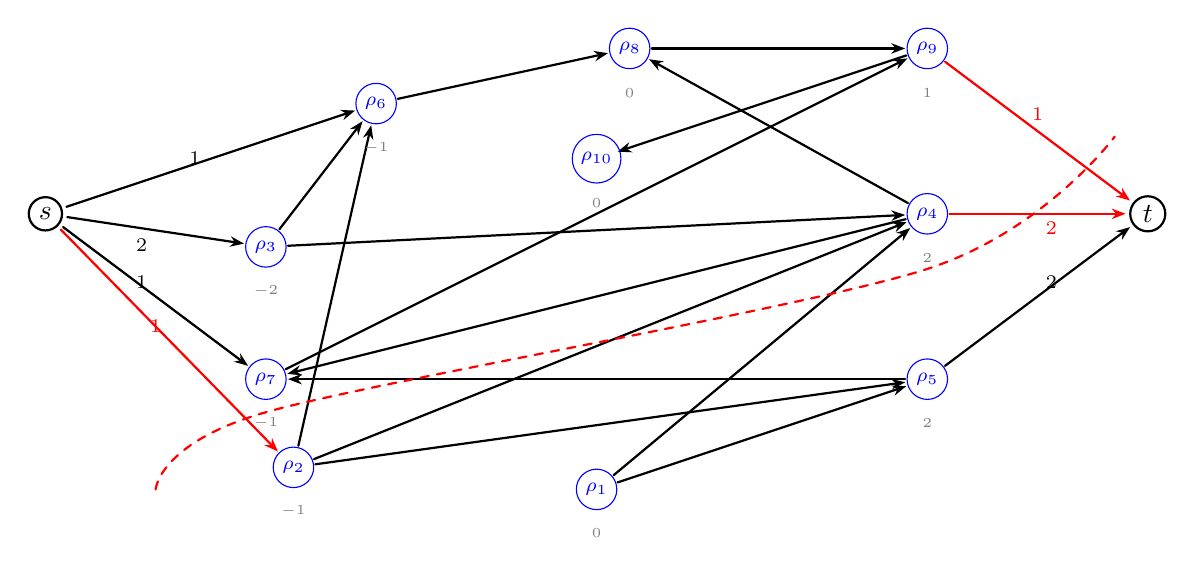
\begin{tikzpicture}[line cap=round,line join=round,scale=1.4]

% Existing edges
\draw[-{Stealth[length=5pt]}, thick, shorten >=8pt, shorten <=8pt] (0,1) -- (3,2);
\draw[-{Stealth[length=5pt]}, thick, shorten >=8pt, shorten <=8pt] (-2.75,1.2) -- (3,3.5);
\draw[-{Stealth[length=5pt]}, thick, shorten >=8pt, shorten <=8pt] (-3,3.2) -- (-2,4.5);
\draw[-{Stealth[length=5pt]}, thick, shorten >=8pt, shorten <=8pt] (-2.75,1.2) -- (-2,4.5);
\draw[-{Stealth[length=5pt]}, thick, shorten >=8pt, shorten <=8pt] (-3,3.2) -- (3,3.5);
\draw[-{Stealth[length=5pt]}, thick, shorten >=8pt, shorten <=8pt] (-2.75,1.2) -- (3,2);
\draw[-{Stealth[length=5pt]}, thick, shorten >=8pt, shorten <=8pt] (0,1) -- (3,3.5);
\draw[-{Stealth[length=5pt]}, thick, shorten >=8pt, shorten <=8pt] (3,3.5) -- (-3,2);
\draw[-{Stealth[length=5pt]}, thick, shorten >=8pt, shorten <=8pt] (3,2)--(-3,2);
\draw[-{Stealth[length=5pt]}, thick, shorten >=8pt, shorten <=8pt] (3,3.5) -- (0.3,5);
\draw[-{Stealth[length=5pt]}, thick, shorten >=8pt, shorten <=8pt] (-2,4.5) -- (0.3,5);
\draw[-{Stealth[length=5pt]}, thick, shorten >=8pt, shorten <=8pt] (-3,2) -- (3,5);
\draw[-{Stealth[length=5pt]}, thick, shorten >=8pt, shorten <=8pt] (0.3,5) -- (3,5);
\draw[-{Stealth[length=5pt]}, thick, shorten >=8pt, shorten <=8pt] (3,5) -- (0,4);

% Nodes with weights
\begin{scriptsize}
\foreach \x/\y/\label/\weight in {
  0/1/\rho_1/0,
  -2.75/1.2/\rho_2/-1,
  -3/3.2/\rho_3/-2,
  3/2/\rho_5/2,
  3/3.5/\rho_4/2,
  -2/4.5/\rho_6/-1,
  -3/2/\rho_7/-1,
  0.3/5/\rho_8/0,
  3/5/\rho_9/1,
  0/4/\rho_{10}/0
} {
  \node[draw=blue, circle, inner sep=2pt, text=blue] at (\x,\y) {$\label$};
  \node[gray] at (\x,\y-0.4) {\tiny $\weight$};
}
\end{scriptsize}

% New s and t nodes
\node[draw=black, circle, inner sep=2pt, text=black, thick] at (-5,3.5) {$s$};
\node[draw=black, circle, inner sep=2pt, text=black, thick] at (5,3.5) {$t$};

% Edges from s to selected nodes
\draw[red, -{Stealth[length=5pt]}, thick, shorten >=8pt, shorten <=8pt](-5,3.5) -- (-2.75,1.2)
  node[midway, above left=-1pt] {\scriptsize 1}; % to rho_2
\draw[-{Stealth[length=5pt]}, thick, shorten >=8pt, shorten <=8pt] (-5,3.5) -- (-3,3.2)
  node[midway, below left=-1pt] {\scriptsize 2}; % to rho_3
\draw[-{Stealth[length=5pt]}, thick, shorten >=8pt, shorten <=8pt] (-5,3.5) -- (-2,4.5)
  node[midway, left] {\scriptsize 1}; % to rho_6
\draw[-{Stealth[length=5pt]}, thick, shorten >=8pt, shorten <=8pt] (-5,3.5) -- (-3,2)
  node[midway, above left=-1pt] {\scriptsize 1}; % to rho_7

% Edges from selected nodes to t
\draw[-{Stealth[length=5pt]}, thick, shorten >=8pt, shorten <=8pt] (3,2) -- (5,3.5)
  node[midway, above right=-1pt] {\scriptsize 2}; % from rho_5
\draw[red, -{Stealth[length=5pt]}, thick, shorten >=8pt, shorten <=8pt] (3,3.5) -- (5,3.5)
  node[midway, below right=-1pt] {\scriptsize 2}; % from rho_4
\draw[red, -{Stealth[length=5pt]}, thick, shorten >=8pt, shorten <=8pt] (3,5) -- (5,3.5)
  node[midway, above] {\scriptsize 1}; % from rho_9

% Cut line (dashed red)
\draw[dashed, red, thick, smooth] plot coordinates {
  (-4,1)
  (-3,1.7)
  (3,3)
  (4.7,4.2)
};

\end{tikzpicture}

Poset $(\rho_1, \rho_2, \rho_5)$ with sum $+1$

\end{frame}


% \begin{frame}{Proof}
%     Let $V^+$ and $V^-$ be the set of sets of positive and negative nodes respectively in $P'$
%     \medskip
    
%     $N(W)$ set of all negative predecessors of any subset $W$ of $V^+$. \pause

%     \medskip
%     Any negative node in a maximum-weight closed subset $C$ of $P'$ must precede at least one positive node in $C$, and hence a maximum-weight closed subset of $P'$ can
% be defined as a subset $W \subseteq V^+$ which maximizes the quantity $w(W) - | w(N(W))|$
% over all subsets $W$ of $V^+$\pause
%     \medskip


% It is same as the subset which minimizes $w(V^+)-(w(W)-|w(N(W))|)$
% \pause

% Hence we can solve finding maximum weight closed subset can be solved by minimizing $w(V^+-W)+|w(N(W))|$ over all subset of $V^+$
% \end{frame}
% \begin{frame}{Proof}
%     Let $W$ be an arbitary subset of $V^+$ for the graph $P'(s,t)$\pause
% \medskip

%     if every edge from $s$ to node in $N(W)$ is cut and every edge from $V^+-W$ to $t$ is also cut then all path from $s$ to $t$ is also cut \pause
% \medskip

%     Hence $w(X)\leq w(V^+-W)+|w(N(W))|$ for any $W\subseteq V^+$
% \end{frame}
% \begin{frame}{Proof}
%     Let $W^*\subseteq V^+$ consist of positive nodes whose edges to $t$ are uncut by $X$ \pause
% \medskip

%     Since $X$ is a $s-t$ min-cut of finite capacity and all original edges are of capacity $\infty$
%     \pause
%     \medskip
    
%     By definition $X$ cuts all edges to $t$ from nodes in $V^+-W^*$  and edges from $s$ to $N(W^*)$

%     Hence 
%     \[w(X)=w(V^+-W^*)+|w(N(W^*))|\leq w(V^+-W)+|w(N(W))|\]

%     for an arbitrary $W\subseteq V^+$ and theorem is proved
% \end{frame}
% \begin{frame}{Sparse sub-graph}
%     Sub-graph consisting of same nodes but only the edges of the form
%     \begin{itemize}
%         \item  If $(m, w)$ is a member of a rotation, say $\pi$, and $w'$ is the first B below $w$ in $m$’s list such that $(m, w')$ is a member of some other rotation, say $\rho$, then $P'$ contains a directed edge from $\pi$ to $\rho$.
%         \item If $(m, w')$ is not a member of any rotation, but is eliminated by some rotation, say $\pi$, and $w$ is the first B above $w'$ in $m$’s list such that $(m, w)$ is a member of some rotation, say $\rho$, then $P'$ contains a directed edge from $\pi$ to $\rho$.

%     \end{itemize}
% \end{frame}
% \begin{frame}{Lemma}
%     \begin{lemma}
%         $P'$ has at most $O(n')$ edges, and, given the rotations, $P'$ can be constructed in $O(n^2)$-time.
%     \end{lemma}\pause
%     Each creation of an edge in $P'$ is associated with a pair $(m, w')$. But no pair is associated more than once, so $P'$ can have at most $O(n^2)$ edges.

% \end{frame}



















% \begin{lemma}
%     The minimum cut in $P'(s, t)$ has capacity bounded by $O(n^2)$
    
% \end{lemma}
% Min cut is bounded by $\sum_{i\in V^+}w(\rho_i)$

%     involve positive part from B side  and negative part from A side
%     $\sum_{i\in V^+}w(\rho_i)\le\sum_i W(\rho_i)$

%     $W(\rho_i)$ is the number of pairs eliminated hence bounded by $O(n^2)$
    
% \end{frame}
\begin{frame}{Complexity Analysis}
  \begin{itemize}
    \item \textbf{Finding all rotations:} \( O(n^3) \)
    \item \textbf{Finding minimum \( s \)-\( t \) cut:} \( O(n^4) \)
    \item \textbf{Maximum-weight closed subset via cut:} \( O(n^2) \)
    \item \textbf{Rotation elimination:} \( O(n^2) \)
  \end{itemize}

  \vspace{10pt}
  \textit{Note:} Any improvement in flow computation directly improves the overall bound.

  \vspace{10pt}
  \textbf{Overall complexity:} \( \boxed{O(n^4)} \)
\end{frame}




\end{document}